\apendice{Especificación de diseño}

\section{Introducción}
En esta sección detallaremos el diseño procedimental y el arquitectónico.

\section{Diseño procedimental}
En este apartado veremos el diseño interno del proyecto, especificando los detalles de los diferentes algoritmos. En este caso nos vamos a ayudar de un diagrama de secuencias que explicará el caso más completo que se podría dar en el proyecto.
\begin{figure}[!h]
	\centering
	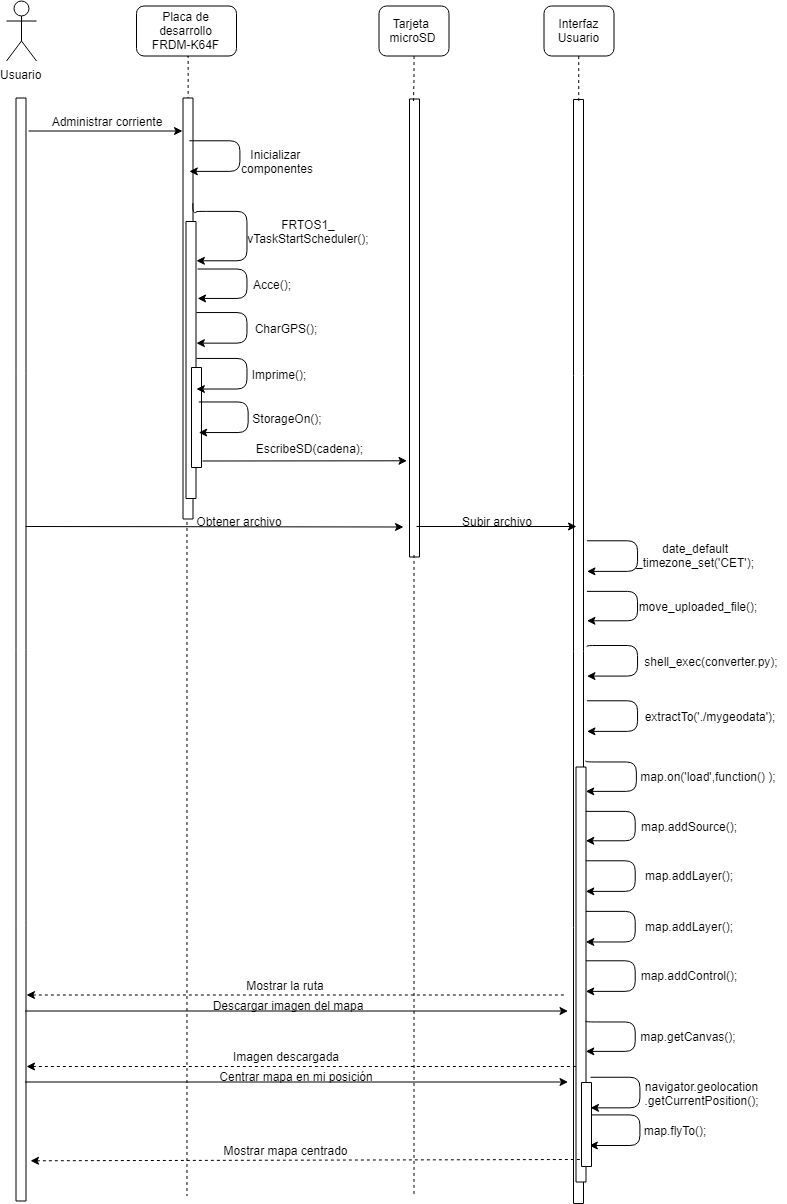
\includegraphics[width=1\textwidth]{diagramasecuencia.PNG}
	\caption{Diagrama de secuencias del proyecto.}\label{fig:diagramasecuencia.PNG}
\end{figure}
\FloatBarrier

\section{Diseño arquitectónico}
En esta sección veremos como se relacionan los diferentes módulos. Desglosaremos el diseño arquitectónico en dos secciones ya que contamos con dos partes claramente diferenciadas.

\subsection{Sistema operativo a tiempo real (RTOS)}
La arquitectura de programación utilizada en el funcionamiento de la placa de desarrollo es comúnmente denominada como ``Sistema operativo a tiempo real'' o RTOS \cite{arquitectura}. Usada en proyectos donde la complejidad es alta y es imprescindible la inclusión de requerimientos de tiempo real, el sistema operativo se encarga de decidir en que momento se debe ejecutar cada tarea a través de interrupciones también autogestionadas. En nuestro caso distinguimos las tareas de almacenar en la cadena los datos enviados por el GPS, la de comprobar los valores del acelerómetro para parar la escritura de datos en caso necesario y la de imprimir los caracteres de la cadena. 

En cuanto se le transmite corriente a la placa, ejecuta el código que alberga en la memoria flash, inicializa los componentes, las tareas y por último, el sistema operativo de tiempo real que las administra.
\imagen{arquitectura.PNG}{Diagrama básico de la arquitectura RTOS.\cite{arquitectura}}

\subsection{Modelo Vista Controlador}
El patrón utilizado para la interfaz web ha sido MVC\cite{mvc}. Se trata de uno de los diseños más usados y separa la vista respecto a la lógica de la aplicación. Intervienen en este diseño 3 componentes:
\begin{itemize}
\tightlist
\item
    \textbf{Modelo:} Se encarga de los datos y maneja la información con la que funciona el proyecto. También conocida como lógica de negocio. En nuestro caso se trata de la API de Mapbox y la de MyGeoData.
\item
    \textbf{Vista:} Se trata de la interfaz, la parte más visible a través de la cual el usuario solicita las acciones y donde se muestra la información. Nuestra página web cumpliría con esta misión mostrando los datos, en este caso la ruta del usuario en el mapa de la forma que él ha especificado.
\item
    \textbf{Controlador:} Es el intermediario entre los dos anteriores, recoge las peticiones del usuario para pasárselas al modelo y devuelve la información a la vista que ha transmitido éste. En nuestro proyecto cobra un papel relevante al ser el encargado de recoger el archivo al usuario, convertirlo y pasárselo al modelo con la configuración solicitada, para que éste después nos devuelva la información que debe ser mostrada en base a los datos aportados.
\end{itemize}
\imagen{mvc.PNG}{Comportamiento de los 3 componentes.\cite{mvcimg}}






